% Created by tikzDevice version 0.12 on 2019-01-03 18:24:23
% !TEX encoding = UTF-8 Unicode
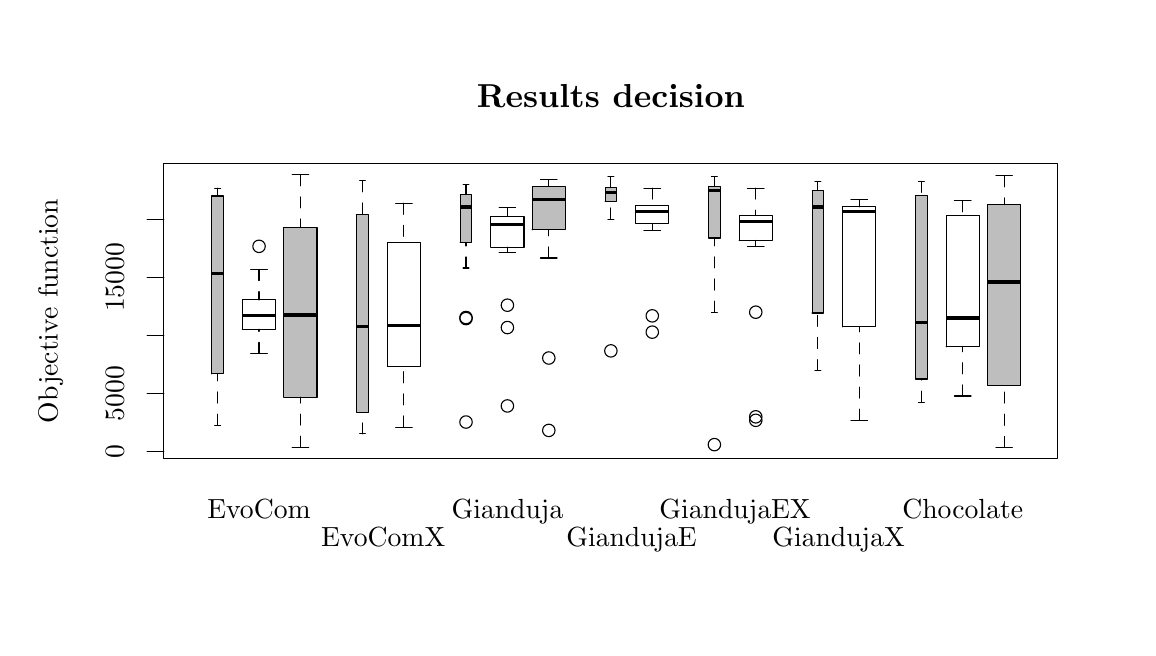
\begin{tikzpicture}[x=1pt,y=1pt]
\definecolor{fillColor}{RGB}{255,255,255}
\path[use as bounding box,fill=fillColor,fill opacity=0.00] (0,0) rectangle (397.48,216.81);
\begin{scope}
\path[clip] ( 49.20, 61.20) rectangle (372.28,167.61);
\definecolor{fillColor}{RGB}{190,190,190}

\path[fill=fillColor] ( 66.55, 91.73) --
	( 70.74, 91.73) --
	( 70.74,155.98) --
	( 66.55,155.98) --
	cycle;
\definecolor{drawColor}{RGB}{0,0,0}

\path[draw=drawColor,line width= 1.2pt,line join=round] ( 66.55,127.90) -- ( 70.74,127.90);

\path[draw=drawColor,line width= 0.4pt,dash pattern=on 4pt off 4pt ,line join=round,line cap=round] ( 68.64, 73.19) -- ( 68.64, 91.73);

\path[draw=drawColor,line width= 0.4pt,dash pattern=on 4pt off 4pt ,line join=round,line cap=round] ( 68.64,158.79) -- ( 68.64,155.98);

\path[draw=drawColor,line width= 0.4pt,line join=round,line cap=round] ( 67.60, 73.19) -- ( 69.69, 73.19);

\path[draw=drawColor,line width= 0.4pt,line join=round,line cap=round] ( 67.60,158.79) -- ( 69.69,158.79);

\path[draw=drawColor,line width= 0.4pt,line join=round,line cap=round] ( 66.55, 91.73) --
	( 70.74, 91.73) --
	( 70.74,155.98) --
	( 66.55,155.98) --
	( 66.55, 91.73);
\definecolor{fillColor}{RGB}{255,255,255}

\path[fill=fillColor] ( 77.62,107.82) --
	( 89.59,107.82) --
	( 89.59,118.45) --
	( 77.62,118.45) --
	cycle;

\path[draw=drawColor,line width= 1.2pt,line join=round] ( 77.62,112.76) -- ( 89.59,112.76);

\path[draw=drawColor,line width= 0.4pt,dash pattern=on 4pt off 4pt ,line join=round,line cap=round] ( 83.60, 99.08) -- ( 83.60,107.82);

\path[draw=drawColor,line width= 0.4pt,dash pattern=on 4pt off 4pt ,line join=round,line cap=round] ( 83.60,129.42) -- ( 83.60,118.45);

\path[draw=drawColor,line width= 0.4pt,line join=round,line cap=round] ( 80.61, 99.08) -- ( 86.59, 99.08);

\path[draw=drawColor,line width= 0.4pt,line join=round,line cap=round] ( 80.61,129.42) -- ( 86.59,129.42);

\path[draw=drawColor,line width= 0.4pt,line join=round,line cap=round] ( 77.62,107.82) --
	( 89.59,107.82) --
	( 89.59,118.45) --
	( 77.62,118.45) --
	( 77.62,107.82);

\path[draw=drawColor,line width= 0.4pt,line join=round,line cap=round] ( 83.60,137.80) circle (  2.25);
\definecolor{fillColor}{RGB}{190,190,190}

\path[fill=fillColor] ( 92.58, 83.30) --
	(104.54, 83.30) --
	(104.54,144.75) --
	( 92.58,144.75) --
	cycle;

\path[draw=drawColor,line width= 1.2pt,line join=round] ( 92.58,112.94) -- (104.54,112.94);

\path[draw=drawColor,line width= 0.4pt,dash pattern=on 4pt off 4pt ,line join=round,line cap=round] ( 98.56, 65.17) -- ( 98.56, 83.30);

\path[draw=drawColor,line width= 0.4pt,dash pattern=on 4pt off 4pt ,line join=round,line cap=round] ( 98.56,163.67) -- ( 98.56,144.75);

\path[draw=drawColor,line width= 0.4pt,line join=round,line cap=round] ( 95.57, 65.17) -- (101.55, 65.17);

\path[draw=drawColor,line width= 0.4pt,line join=round,line cap=round] ( 95.57,163.67) -- (101.55,163.67);

\path[draw=drawColor,line width= 0.4pt,line join=round,line cap=round] ( 92.58, 83.30) --
	(104.54, 83.30) --
	(104.54,144.75) --
	( 92.58,144.75) --
	( 92.58, 83.30);

\path[fill=fillColor] (118.90, 77.81) --
	(123.09, 77.81) --
	(123.09,149.27) --
	(118.90,149.27) --
	cycle;

\path[draw=drawColor,line width= 1.2pt,line join=round] (118.90,108.73) -- (123.09,108.73);

\path[draw=drawColor,line width= 0.4pt,dash pattern=on 4pt off 4pt ,line join=round,line cap=round] (121.00, 70.01) -- (121.00, 77.81);

\path[draw=drawColor,line width= 0.4pt,dash pattern=on 4pt off 4pt ,line join=round,line cap=round] (121.00,161.48) -- (121.00,149.27);

\path[draw=drawColor,line width= 0.4pt,line join=round,line cap=round] (119.95, 70.01) -- (122.04, 70.01);

\path[draw=drawColor,line width= 0.4pt,line join=round,line cap=round] (119.95,161.48) -- (122.04,161.48);

\path[draw=drawColor,line width= 0.4pt,line join=round,line cap=round] (118.90, 77.81) --
	(123.09, 77.81) --
	(123.09,149.27) --
	(118.90,149.27) --
	(118.90, 77.81);
\definecolor{fillColor}{RGB}{255,255,255}

\path[fill=fillColor] (129.97, 94.47) --
	(141.94, 94.47) --
	(141.94,139.04) --
	(129.97,139.04) --
	cycle;

\path[draw=drawColor,line width= 1.2pt,line join=round] (129.97,109.20) -- (141.94,109.20);

\path[draw=drawColor,line width= 0.4pt,dash pattern=on 4pt off 4pt ,line join=round,line cap=round] (135.95, 72.49) -- (135.95, 94.47);

\path[draw=drawColor,line width= 0.4pt,dash pattern=on 4pt off 4pt ,line join=round,line cap=round] (135.95,153.38) -- (135.95,139.04);

\path[draw=drawColor,line width= 0.4pt,line join=round,line cap=round] (132.96, 72.49) -- (138.95, 72.49);

\path[draw=drawColor,line width= 0.4pt,line join=round,line cap=round] (132.96,153.38) -- (138.95,153.38);

\path[draw=drawColor,line width= 0.4pt,line join=round,line cap=round] (129.97, 94.47) --
	(141.94, 94.47) --
	(141.94,139.04) --
	(129.97,139.04) --
	(129.97, 94.47);
\definecolor{fillColor}{RGB}{190,190,190}

\path[fill=fillColor] (156.30,139.20) --
	(160.48,139.20) --
	(160.48,156.50) --
	(156.30,156.50) --
	cycle;

\path[draw=drawColor,line width= 1.2pt,line join=round] (156.30,152.04) -- (160.48,152.04);

\path[draw=drawColor,line width= 0.4pt,dash pattern=on 4pt off 4pt ,line join=round,line cap=round] (158.39,129.95) -- (158.39,139.20);

\path[draw=drawColor,line width= 0.4pt,dash pattern=on 4pt off 4pt ,line join=round,line cap=round] (158.39,160.10) -- (158.39,156.50);

\path[draw=drawColor,line width= 0.4pt,line join=round,line cap=round] (157.34,129.95) -- (159.44,129.95);

\path[draw=drawColor,line width= 0.4pt,line join=round,line cap=round] (157.34,160.10) -- (159.44,160.10);

\path[draw=drawColor,line width= 0.4pt,line join=round,line cap=round] (156.30,139.20) --
	(160.48,139.20) --
	(160.48,156.50) --
	(156.30,156.50) --
	(156.30,139.20);

\path[draw=drawColor,line width= 0.4pt,line join=round,line cap=round] (158.39,112.08) circle (  2.25);

\path[draw=drawColor,line width= 0.4pt,line join=round,line cap=round] (158.39, 74.31) circle (  2.25);

\path[draw=drawColor,line width= 0.4pt,line join=round,line cap=round] (158.39,111.69) circle (  2.25);
\definecolor{fillColor}{RGB}{255,255,255}

\path[fill=fillColor] (167.37,137.51) --
	(179.33,137.51) --
	(179.33,148.66) --
	(167.37,148.66) --
	cycle;

\path[draw=drawColor,line width= 1.2pt,line join=round] (167.37,145.68) -- (179.33,145.68);

\path[draw=drawColor,line width= 0.4pt,dash pattern=on 4pt off 4pt ,line join=round,line cap=round] (173.35,135.50) -- (173.35,137.51);

\path[draw=drawColor,line width= 0.4pt,dash pattern=on 4pt off 4pt ,line join=round,line cap=round] (173.35,151.76) -- (173.35,148.66);

\path[draw=drawColor,line width= 0.4pt,line join=round,line cap=round] (170.36,135.50) -- (176.34,135.50);

\path[draw=drawColor,line width= 0.4pt,line join=round,line cap=round] (170.36,151.76) -- (176.34,151.76);

\path[draw=drawColor,line width= 0.4pt,line join=round,line cap=round] (167.37,137.51) --
	(179.33,137.51) --
	(179.33,148.66) --
	(167.37,148.66) --
	(167.37,137.51);

\path[draw=drawColor,line width= 0.4pt,line join=round,line cap=round] (173.35,108.45) circle (  2.25);

\path[draw=drawColor,line width= 0.4pt,line join=round,line cap=round] (173.35, 80.12) circle (  2.25);

\path[draw=drawColor,line width= 0.4pt,line join=round,line cap=round] (173.35,116.53) circle (  2.25);
\definecolor{fillColor}{RGB}{190,190,190}

\path[fill=fillColor] (182.32,143.72) --
	(194.29,143.72) --
	(194.29,159.55) --
	(182.32,159.55) --
	cycle;

\path[draw=drawColor,line width= 1.2pt,line join=round] (182.32,154.68) -- (194.29,154.68);

\path[draw=drawColor,line width= 0.4pt,dash pattern=on 4pt off 4pt ,line join=round,line cap=round] (188.31,133.57) -- (188.31,143.72);

\path[draw=drawColor,line width= 0.4pt,dash pattern=on 4pt off 4pt ,line join=round,line cap=round] (188.31,161.91) -- (188.31,159.55);

\path[draw=drawColor,line width= 0.4pt,line join=round,line cap=round] (185.31,133.57) -- (191.30,133.57);

\path[draw=drawColor,line width= 0.4pt,line join=round,line cap=round] (185.31,161.91) -- (191.30,161.91);

\path[draw=drawColor,line width= 0.4pt,line join=round,line cap=round] (182.32,143.72) --
	(194.29,143.72) --
	(194.29,159.55) --
	(182.32,159.55) --
	(182.32,143.72);

\path[draw=drawColor,line width= 0.4pt,line join=round,line cap=round] (188.31, 71.28) circle (  2.25);

\path[draw=drawColor,line width= 0.4pt,line join=round,line cap=round] (188.31, 97.44) circle (  2.25);

\path[fill=fillColor] (208.65,154.02) --
	(212.84,154.02) --
	(212.84,159.01) --
	(208.65,159.01) --
	cycle;

\path[draw=drawColor,line width= 1.2pt,line join=round] (208.65,157.15) -- (212.84,157.15);

\path[draw=drawColor,line width= 0.4pt,dash pattern=on 4pt off 4pt ,line join=round,line cap=round] (210.74,147.65) -- (210.74,154.02);

\path[draw=drawColor,line width= 0.4pt,dash pattern=on 4pt off 4pt ,line join=round,line cap=round] (210.74,162.96) -- (210.74,159.01);

\path[draw=drawColor,line width= 0.4pt,line join=round,line cap=round] (209.70,147.65) -- (211.79,147.65);

\path[draw=drawColor,line width= 0.4pt,line join=round,line cap=round] (209.70,162.96) -- (211.79,162.96);

\path[draw=drawColor,line width= 0.4pt,line join=round,line cap=round] (208.65,154.02) --
	(212.84,154.02) --
	(212.84,159.01) --
	(208.65,159.01) --
	(208.65,154.02);

\path[draw=drawColor,line width= 0.4pt,line join=round,line cap=round] (210.74,100.02) circle (  2.25);
\definecolor{fillColor}{RGB}{255,255,255}

\path[fill=fillColor] (219.72,146.10) --
	(231.68,146.10) --
	(231.68,152.55) --
	(219.72,152.55) --
	cycle;

\path[draw=drawColor,line width= 1.2pt,line join=round] (219.72,150.26) -- (231.68,150.26);

\path[draw=drawColor,line width= 0.4pt,dash pattern=on 4pt off 4pt ,line join=round,line cap=round] (225.70,143.60) -- (225.70,146.10);

\path[draw=drawColor,line width= 0.4pt,dash pattern=on 4pt off 4pt ,line join=round,line cap=round] (225.70,158.84) -- (225.70,152.55);

\path[draw=drawColor,line width= 0.4pt,line join=round,line cap=round] (222.71,143.60) -- (228.69,143.60);

\path[draw=drawColor,line width= 0.4pt,line join=round,line cap=round] (222.71,158.84) -- (228.69,158.84);

\path[draw=drawColor,line width= 0.4pt,line join=round,line cap=round] (219.72,146.10) --
	(231.68,146.10) --
	(231.68,152.55) --
	(219.72,152.55) --
	(219.72,146.10);

\path[draw=drawColor,line width= 0.4pt,line join=round,line cap=round] (225.70,112.67) circle (  2.25);

\path[draw=drawColor,line width= 0.4pt,line join=round,line cap=round] (225.70,106.79) circle (  2.25);
\definecolor{fillColor}{RGB}{190,190,190}

\path[fill=fillColor] (246.04,140.82) --
	(250.23,140.82) --
	(250.23,159.53) --
	(246.04,159.53) --
	cycle;

\path[draw=drawColor,line width= 1.2pt,line join=round] (246.04,158.09) -- (250.23,158.09);

\path[draw=drawColor,line width= 0.4pt,dash pattern=on 4pt off 4pt ,line join=round,line cap=round] (248.14,114.00) -- (248.14,140.82);

\path[draw=drawColor,line width= 0.4pt,dash pattern=on 4pt off 4pt ,line join=round,line cap=round] (248.14,162.96) -- (248.14,159.53);

\path[draw=drawColor,line width= 0.4pt,line join=round,line cap=round] (247.09,114.00) -- (249.18,114.00);

\path[draw=drawColor,line width= 0.4pt,line join=round,line cap=round] (247.09,162.96) -- (249.18,162.96);

\path[draw=drawColor,line width= 0.4pt,line join=round,line cap=round] (246.04,140.82) --
	(250.23,140.82) --
	(250.23,159.53) --
	(246.04,159.53) --
	(246.04,140.82);

\path[draw=drawColor,line width= 0.4pt,line join=round,line cap=round] (248.14, 66.14) circle (  2.25);
\definecolor{fillColor}{RGB}{255,255,255}

\path[fill=fillColor] (257.11,139.90) --
	(269.08,139.90) --
	(269.08,148.91) --
	(257.11,148.91) --
	cycle;

\path[draw=drawColor,line width= 1.2pt,line join=round] (257.11,146.86) -- (269.08,146.86);

\path[draw=drawColor,line width= 0.4pt,dash pattern=on 4pt off 4pt ,line join=round,line cap=round] (263.09,137.83) -- (263.09,139.90);

\path[draw=drawColor,line width= 0.4pt,dash pattern=on 4pt off 4pt ,line join=round,line cap=round] (263.09,158.84) -- (263.09,148.91);

\path[draw=drawColor,line width= 0.4pt,line join=round,line cap=round] (260.10,137.83) -- (266.09,137.83);

\path[draw=drawColor,line width= 0.4pt,line join=round,line cap=round] (260.10,158.84) -- (266.09,158.84);

\path[draw=drawColor,line width= 0.4pt,line join=round,line cap=round] (257.11,139.90) --
	(269.08,139.90) --
	(269.08,148.91) --
	(257.11,148.91) --
	(257.11,139.90);

\path[draw=drawColor,line width= 0.4pt,line join=round,line cap=round] (263.09,114.00) circle (  2.25);

\path[draw=drawColor,line width= 0.4pt,line join=round,line cap=round] (263.09, 74.93) circle (  2.25);

\path[draw=drawColor,line width= 0.4pt,line join=round,line cap=round] (263.09, 76.19) circle (  2.25);
\definecolor{fillColor}{RGB}{190,190,190}

\path[fill=fillColor] (283.44,113.71) --
	(287.62,113.71) --
	(287.62,158.04) --
	(283.44,158.04) --
	cycle;

\path[draw=drawColor,line width= 1.2pt,line join=round] (283.44,152.04) -- (287.62,152.04);

\path[draw=drawColor,line width= 0.4pt,dash pattern=on 4pt off 4pt ,line join=round,line cap=round] (285.53, 92.86) -- (285.53,113.71);

\path[draw=drawColor,line width= 0.4pt,dash pattern=on 4pt off 4pt ,line join=round,line cap=round] (285.53,161.27) -- (285.53,158.04);

\path[draw=drawColor,line width= 0.4pt,line join=round,line cap=round] (284.48, 92.86) -- (286.58, 92.86);

\path[draw=drawColor,line width= 0.4pt,line join=round,line cap=round] (284.48,161.27) -- (286.58,161.27);

\path[draw=drawColor,line width= 0.4pt,line join=round,line cap=round] (283.44,113.71) --
	(287.62,113.71) --
	(287.62,158.04) --
	(283.44,158.04) --
	(283.44,113.71);
\definecolor{fillColor}{RGB}{255,255,255}

\path[fill=fillColor] (294.51,108.70) --
	(306.47,108.70) --
	(306.47,152.10) --
	(294.51,152.10) --
	cycle;

\path[draw=drawColor,line width= 1.2pt,line join=round] (294.51,150.48) -- (306.47,150.48);

\path[draw=drawColor,line width= 0.4pt,dash pattern=on 4pt off 4pt ,line join=round,line cap=round] (300.49, 74.93) -- (300.49,108.70);

\path[draw=drawColor,line width= 0.4pt,dash pattern=on 4pt off 4pt ,line join=round,line cap=round] (300.49,154.56) -- (300.49,152.10);

\path[draw=drawColor,line width= 0.4pt,line join=round,line cap=round] (297.50, 74.93) -- (303.48, 74.93);

\path[draw=drawColor,line width= 0.4pt,line join=round,line cap=round] (297.50,154.56) -- (303.48,154.56);

\path[draw=drawColor,line width= 0.4pt,line join=round,line cap=round] (294.51,108.70) --
	(306.47,108.70) --
	(306.47,152.10) --
	(294.51,152.10) --
	(294.51,108.70);
\definecolor{fillColor}{RGB}{190,190,190}

\path[fill=fillColor] (320.83, 89.87) --
	(325.02, 89.87) --
	(325.02,156.16) --
	(320.83,156.16) --
	cycle;

\path[draw=drawColor,line width= 1.2pt,line join=round] (320.83,110.17) -- (325.02,110.17);

\path[draw=drawColor,line width= 0.4pt,dash pattern=on 4pt off 4pt ,line join=round,line cap=round] (322.92, 81.45) -- (322.92, 89.87);

\path[draw=drawColor,line width= 0.4pt,dash pattern=on 4pt off 4pt ,line join=round,line cap=round] (322.92,161.27) -- (322.92,156.16);

\path[draw=drawColor,line width= 0.4pt,line join=round,line cap=round] (321.88, 81.45) -- (323.97, 81.45);

\path[draw=drawColor,line width= 0.4pt,line join=round,line cap=round] (321.88,161.27) -- (323.97,161.27);

\path[draw=drawColor,line width= 0.4pt,line join=round,line cap=round] (320.83, 89.87) --
	(325.02, 89.87) --
	(325.02,156.16) --
	(320.83,156.16) --
	(320.83, 89.87);
\definecolor{fillColor}{RGB}{255,255,255}

\path[fill=fillColor] (331.90,101.44) --
	(343.87,101.44) --
	(343.87,148.78) --
	(331.90,148.78) --
	cycle;

\path[draw=drawColor,line width= 1.2pt,line join=round] (331.90,111.88) -- (343.87,111.88);

\path[draw=drawColor,line width= 0.4pt,dash pattern=on 4pt off 4pt ,line join=round,line cap=round] (337.88, 83.72) -- (337.88,101.44);

\path[draw=drawColor,line width= 0.4pt,dash pattern=on 4pt off 4pt ,line join=round,line cap=round] (337.88,154.26) -- (337.88,148.78);

\path[draw=drawColor,line width= 0.4pt,line join=round,line cap=round] (334.89, 83.72) -- (340.87, 83.72);

\path[draw=drawColor,line width= 0.4pt,line join=round,line cap=round] (334.89,154.26) -- (340.87,154.26);

\path[draw=drawColor,line width= 0.4pt,line join=round,line cap=round] (331.90,101.44) --
	(343.87,101.44) --
	(343.87,148.78) --
	(331.90,148.78) --
	(331.90,101.44);
\definecolor{fillColor}{RGB}{190,190,190}

\path[fill=fillColor] (346.86, 87.60) --
	(358.82, 87.60) --
	(358.82,152.84) --
	(346.86,152.84) --
	cycle;

\path[draw=drawColor,line width= 1.2pt,line join=round] (346.86,124.85) -- (358.82,124.85);

\path[draw=drawColor,line width= 0.4pt,dash pattern=on 4pt off 4pt ,line join=round,line cap=round] (352.84, 65.14) -- (352.84, 87.60);

\path[draw=drawColor,line width= 0.4pt,dash pattern=on 4pt off 4pt ,line join=round,line cap=round] (352.84,163.26) -- (352.84,152.84);

\path[draw=drawColor,line width= 0.4pt,line join=round,line cap=round] (349.85, 65.14) -- (355.83, 65.14);

\path[draw=drawColor,line width= 0.4pt,line join=round,line cap=round] (349.85,163.26) -- (355.83,163.26);

\path[draw=drawColor,line width= 0.4pt,line join=round,line cap=round] (346.86, 87.60) --
	(358.82, 87.60) --
	(358.82,152.84) --
	(346.86,152.84) --
	(346.86, 87.60);
\end{scope}
\begin{scope}
\path[clip] (  0.00,  0.00) rectangle (397.48,216.81);
\definecolor{drawColor}{RGB}{0,0,0}

\node[text=drawColor,rotate= 90.00,anchor=base,inner sep=0pt, outer sep=0pt, scale=  1.00] at ( 10.80,114.41) {Objective function};
\end{scope}
\begin{scope}
\path[clip] (  0.00,  0.00) rectangle (397.48,216.81);
\definecolor{drawColor}{RGB}{0,0,0}

\node[text=drawColor,anchor=base,inner sep=0pt, outer sep=0pt, scale=  1.00] at ( 83.60, 39.60) {EvoCom};

\node[text=drawColor,anchor=base,inner sep=0pt, outer sep=0pt, scale=  1.00] at (173.35, 39.60) {Gianduja};

\node[text=drawColor,anchor=base,inner sep=0pt, outer sep=0pt, scale=  1.00] at (255.62, 39.60) {GiandujaEX};

\node[text=drawColor,anchor=base,inner sep=0pt, outer sep=0pt, scale=  1.00] at (337.88, 39.60) {Chocolate};

\node[text=drawColor,anchor=base,inner sep=0pt, outer sep=0pt, scale=  1.00] at (128.48, 29.27) {EvoComX};

\node[text=drawColor,anchor=base,inner sep=0pt, outer sep=0pt, scale=  1.00] at (218.22, 29.27) {GiandujaE};

\node[text=drawColor,anchor=base,inner sep=0pt, outer sep=0pt, scale=  1.00] at (293.01, 29.27) {GiandujaX};
\end{scope}
\begin{scope}
\path[clip] (  0.00,  0.00) rectangle (397.48,216.81);
\definecolor{drawColor}{RGB}{0,0,0}

\node[text=drawColor,anchor=base,inner sep=0pt, outer sep=0pt, scale=  1.20] at (210.74,188.07) {\bfseries Results decision};
\end{scope}
\begin{scope}
\path[clip] (  0.00,  0.00) rectangle (397.48,216.81);
\definecolor{drawColor}{RGB}{0,0,0}

\path[draw=drawColor,line width= 0.4pt,line join=round,line cap=round] ( 49.20, 63.64) -- ( 49.20,147.56);

\path[draw=drawColor,line width= 0.4pt,line join=round,line cap=round] ( 49.20, 63.64) -- ( 43.20, 63.64);

\path[draw=drawColor,line width= 0.4pt,line join=round,line cap=round] ( 49.20, 84.62) -- ( 43.20, 84.62);

\path[draw=drawColor,line width= 0.4pt,line join=round,line cap=round] ( 49.20,105.60) -- ( 43.20,105.60);

\path[draw=drawColor,line width= 0.4pt,line join=round,line cap=round] ( 49.20,126.58) -- ( 43.20,126.58);

\path[draw=drawColor,line width= 0.4pt,line join=round,line cap=round] ( 49.20,147.56) -- ( 43.20,147.56);

\node[text=drawColor,rotate= 90.00,anchor=base,inner sep=0pt, outer sep=0pt, scale=  1.00] at ( 34.80, 63.64) {0};

\node[text=drawColor,rotate= 90.00,anchor=base,inner sep=0pt, outer sep=0pt, scale=  1.00] at ( 34.80, 84.62) {5000};

\node[text=drawColor,rotate= 90.00,anchor=base,inner sep=0pt, outer sep=0pt, scale=  1.00] at ( 34.80,126.58) {15000};

\path[draw=drawColor,line width= 0.4pt,line join=round,line cap=round] ( 49.20, 61.20) --
	(372.28, 61.20) --
	(372.28,167.61) --
	( 49.20,167.61) --
	( 49.20, 61.20);
\end{scope}
\end{tikzpicture}
